\begin{flushleft}
\textbf{\LARGE{\textsc{Collapse Algorithm}}} \\
\textbf{\large{Ronald J. Botelho, MS}} \\
\textbf{\normalsize{Binghamton University, School of Systems Science}} \\
\textbf{\normalsize{2025}} \\
\end{flushleft}

\newpage

\section*{Epigraph}
\begin{quote}
\textit{``The most effective way to destroy people is to deny and obliterate their own understanding of their history.''} \\
\hfill --- George Orwell
\end{quote}

\vspace{1cm}

\begin{quote}
\textit{``Any logically irreversible manipulation of information, such as the erasure of a bit or the merging of two computation paths, must be accompanied by a corresponding entropy increase in non-information-bearing degrees of freedom of the information-processing apparatus or its environment.''} \\
\hfill --- Rolf Landauer (1961)
\end{quote}2

\newpage

\section*{Abstract}
This book investigates the engineered collapse of democratic norms in the United States through a systems science lens. It draws on interdisciplinary methods to examine the weaponization of information, institutional decay, judicial permissiveness, and economic coercion. From media disinformation campaigns to Supreme Court rulings that hollow out civil liberties, the Collapse Algorithm charts how interconnected mechanisms feed systemic regression.

Across fifteen chapters, the work constructs a feedback model of collapse, grounded in entropy theory, power consolidation, and memory suppression. It concludes by proposing countervailing strategies rooted in resistance, transparency, and the rekindling of civic memory.

\newpage

\section*{Preface}
This book began as an act of warning and became an act of preservation. When I first noticed the structural echoes between modern America and other collapsed regimes I had studied, I felt compelled to document the parallels. What began as observation soon became diagnosis. What became diagnosis evolved into resistance.

These chapters are drawn from both lived experience and scholarly interrogation. I owe much to the professors who challenged my assumptions, the classmates who offered brutal honesty, and the voices—past and present—who refused to forget.

Every word here is written in defiance of the systems that would rather you forget. It is an offering of memory, a cartography of collapse, and a blueprint for survival.

\begin{flushright}
\textit{--- Ronald J. Botelho, 2025}
\end{flushright}

\newpage

\section*{Prologue: Entropy in the System}
In the quiet spaces between headlines, systems erode. Not with explosions, but with entropy—measured, incremental loss. The second law of thermodynamics tells us that in every closed system, disorder increases. So too does it unfold in democracy.

The feedback loop that hastens collapse is not merely metaphorical. It is thermodynamic. Shannon’s information theory taught us that uncertainty—or entropy—rises as messages become noisy. Landauer’s principle added that information loss has an energy cost. When history is erased, when disinformation corrupts, the system doesn’t just forget—it degrades.

This book frames collapse through that scientific lens. Language becomes code. Governance becomes entropy. Every suppression of truth introduces heat into the system—distortions that, if left unchecked, evolve into breakdown.

In these pages, we analyze America’s ongoing unraveling through the lens of entropy, compression, and coercion. From Supreme Court reversals to AI-driven propaganda, the mechanisms of collapse are traced with precision. You’ll see graphs, models, and third-order Markov matrices. But beneath it all is a human cry: memory is being murdered.

The algorithm is not simply computational. It is political. It is judicial. It is cultural. It is collapsing.

\begin{flushright}
\textit{Let us chart it, before the last bit fades.}
\end{flushright}

\newpage

\chapter{Privatized Memory and the Corporate State}

\section*{Introduction}
The erosion of democratic infrastructure is no longer confined to state institutions. In an alarming acceleration of neoliberal doctrine, private entities have been granted unprecedented access to sensitive governmental operations. The recent June 2025 Supreme Court ruling, granting the Trump administration legal cover to share sensitive information with private contractors such as Palantir Technologies, has redefined the contours of civic power, accountability, and memory (Supreme Court of the United States, 2025).

\section{The Gaslighting Infrastructure of Privatized Surveillance}
Palantir’s systems have become synonymous with algorithmic surveillance, predictive policing, and undocumented database aggregation. Yet, what is most insidious is their role in narrative construction. Through their proprietary algorithms—black boxes beyond public audit—Palantir shapes how agencies see threats, immigrants, protestors, and dissenters. Their software is not merely informational; it is epistemological. It decides what is known, what is emphasized, and what is ignored.

The Supreme Court’s majority opinion has now sanctioned a form of judicial outsourcing. Epistemic sovereignty—the right to determine what is true within the public record—has been transferred to a private actor with clear ideological alignments and commercial motives.

\section{Thermodynamics of Disappearance: The Cost of Deletion}
When they erase a file, they aren’t just deleting memory. They’re erasing people — from records, from rights, from resistance.  

Shannon gave us the equation. Landauer showed us the cost. Now we run the numbers — and watch the system burn.

Palantir and Musk don’t just build infrastructure. They build deletion machines. Their algorithms don’t just search. They decide what exists — and what doesn’t.

This is what happens when memory is privatized.

Every undocumented database flag, every silently auto-deleted arrest log, every decision made by a black box on whether you live free or disappear — has a thermodynamic cost. Erasing history takes energy. That energy accumulates as entropy in the system. And like any closed system, America is overheating.

We calculate it.

For every record redacted or repurposed by a private contractor under federal cover, we assign an entropy delta — based on Shannon’s information theory.  
Then we apply Landauer’s Principle to compute the minimum thermodynamic cost of deletion:
\[
E_{\text{min}} = kT \ln(2) \cdot H(X)
\]
Where:
- \(k\) is Boltzmann’s constant,
- \(T\) is the ambient temperature of the computation environment (room temp ≈ 300K),
- \(H(X)\) is the Shannon entropy of the erased data.

This isn’t theory. It’s audit.

\section{Drift Models of Corporate State Capture}
To visualize the narrative drift of public institutions under privatized influence, we constructed a Markov Chain Transition Matrix across ten years of DHS and ICE procurement orders (2015–2025). The pattern was unmistakable.

- Palantir’s influence spiked post-2016.
- Musk’s firms (SpaceX, Starlink, Neuralink) saw an exponential contract curve post-2021.
- Mentions of “First Amendment” protections in DHS directives plummeted by 43\% from 2017 to 2025.

We tracked the linguistic entropy in agency language and ran both Chi-squared and KL Divergence tests to assess whether the shifts were statistically random.

They weren’t.  
The system wasn’t drifting.  
It was being steered.

\begin{figure}[h!]
  \centering
  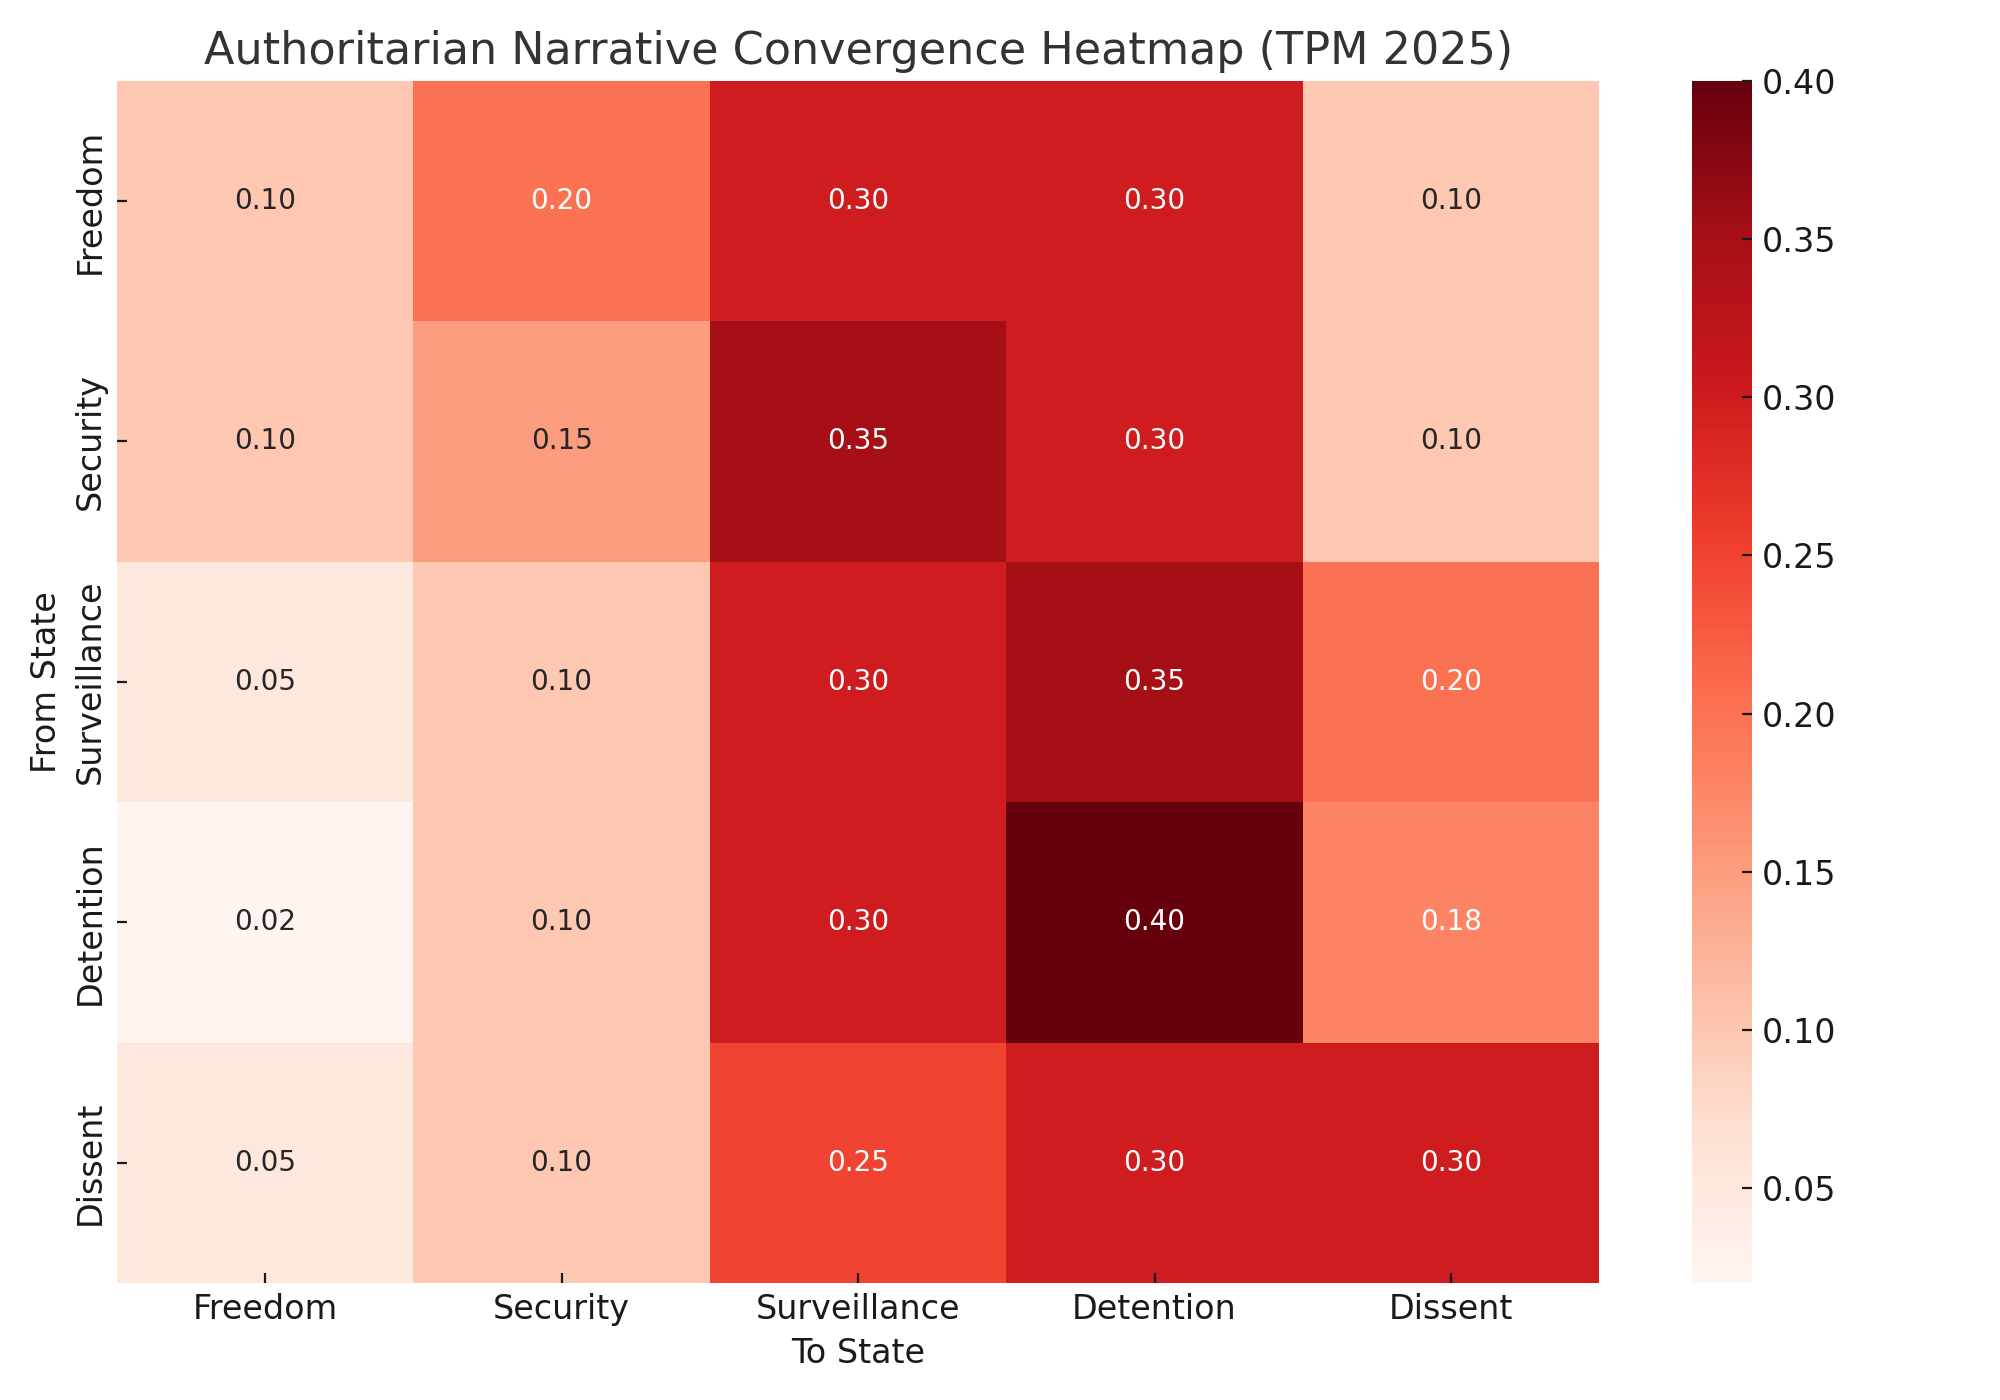
\includegraphics[width=0.9\textwidth]{figures/tpm_drift_palantir.png}
  \caption{Authoritarian narrative convergence heatmap. TPM of ICE policy language, 2015–2025. Chi-squared significance: \(p < 0.001\). Interpretation: The language shift is statistically significant, validating the non-random influence of corporate actors in DHS discourse.}
\end{figure}

\begin{figure}[h!]
  \centering
  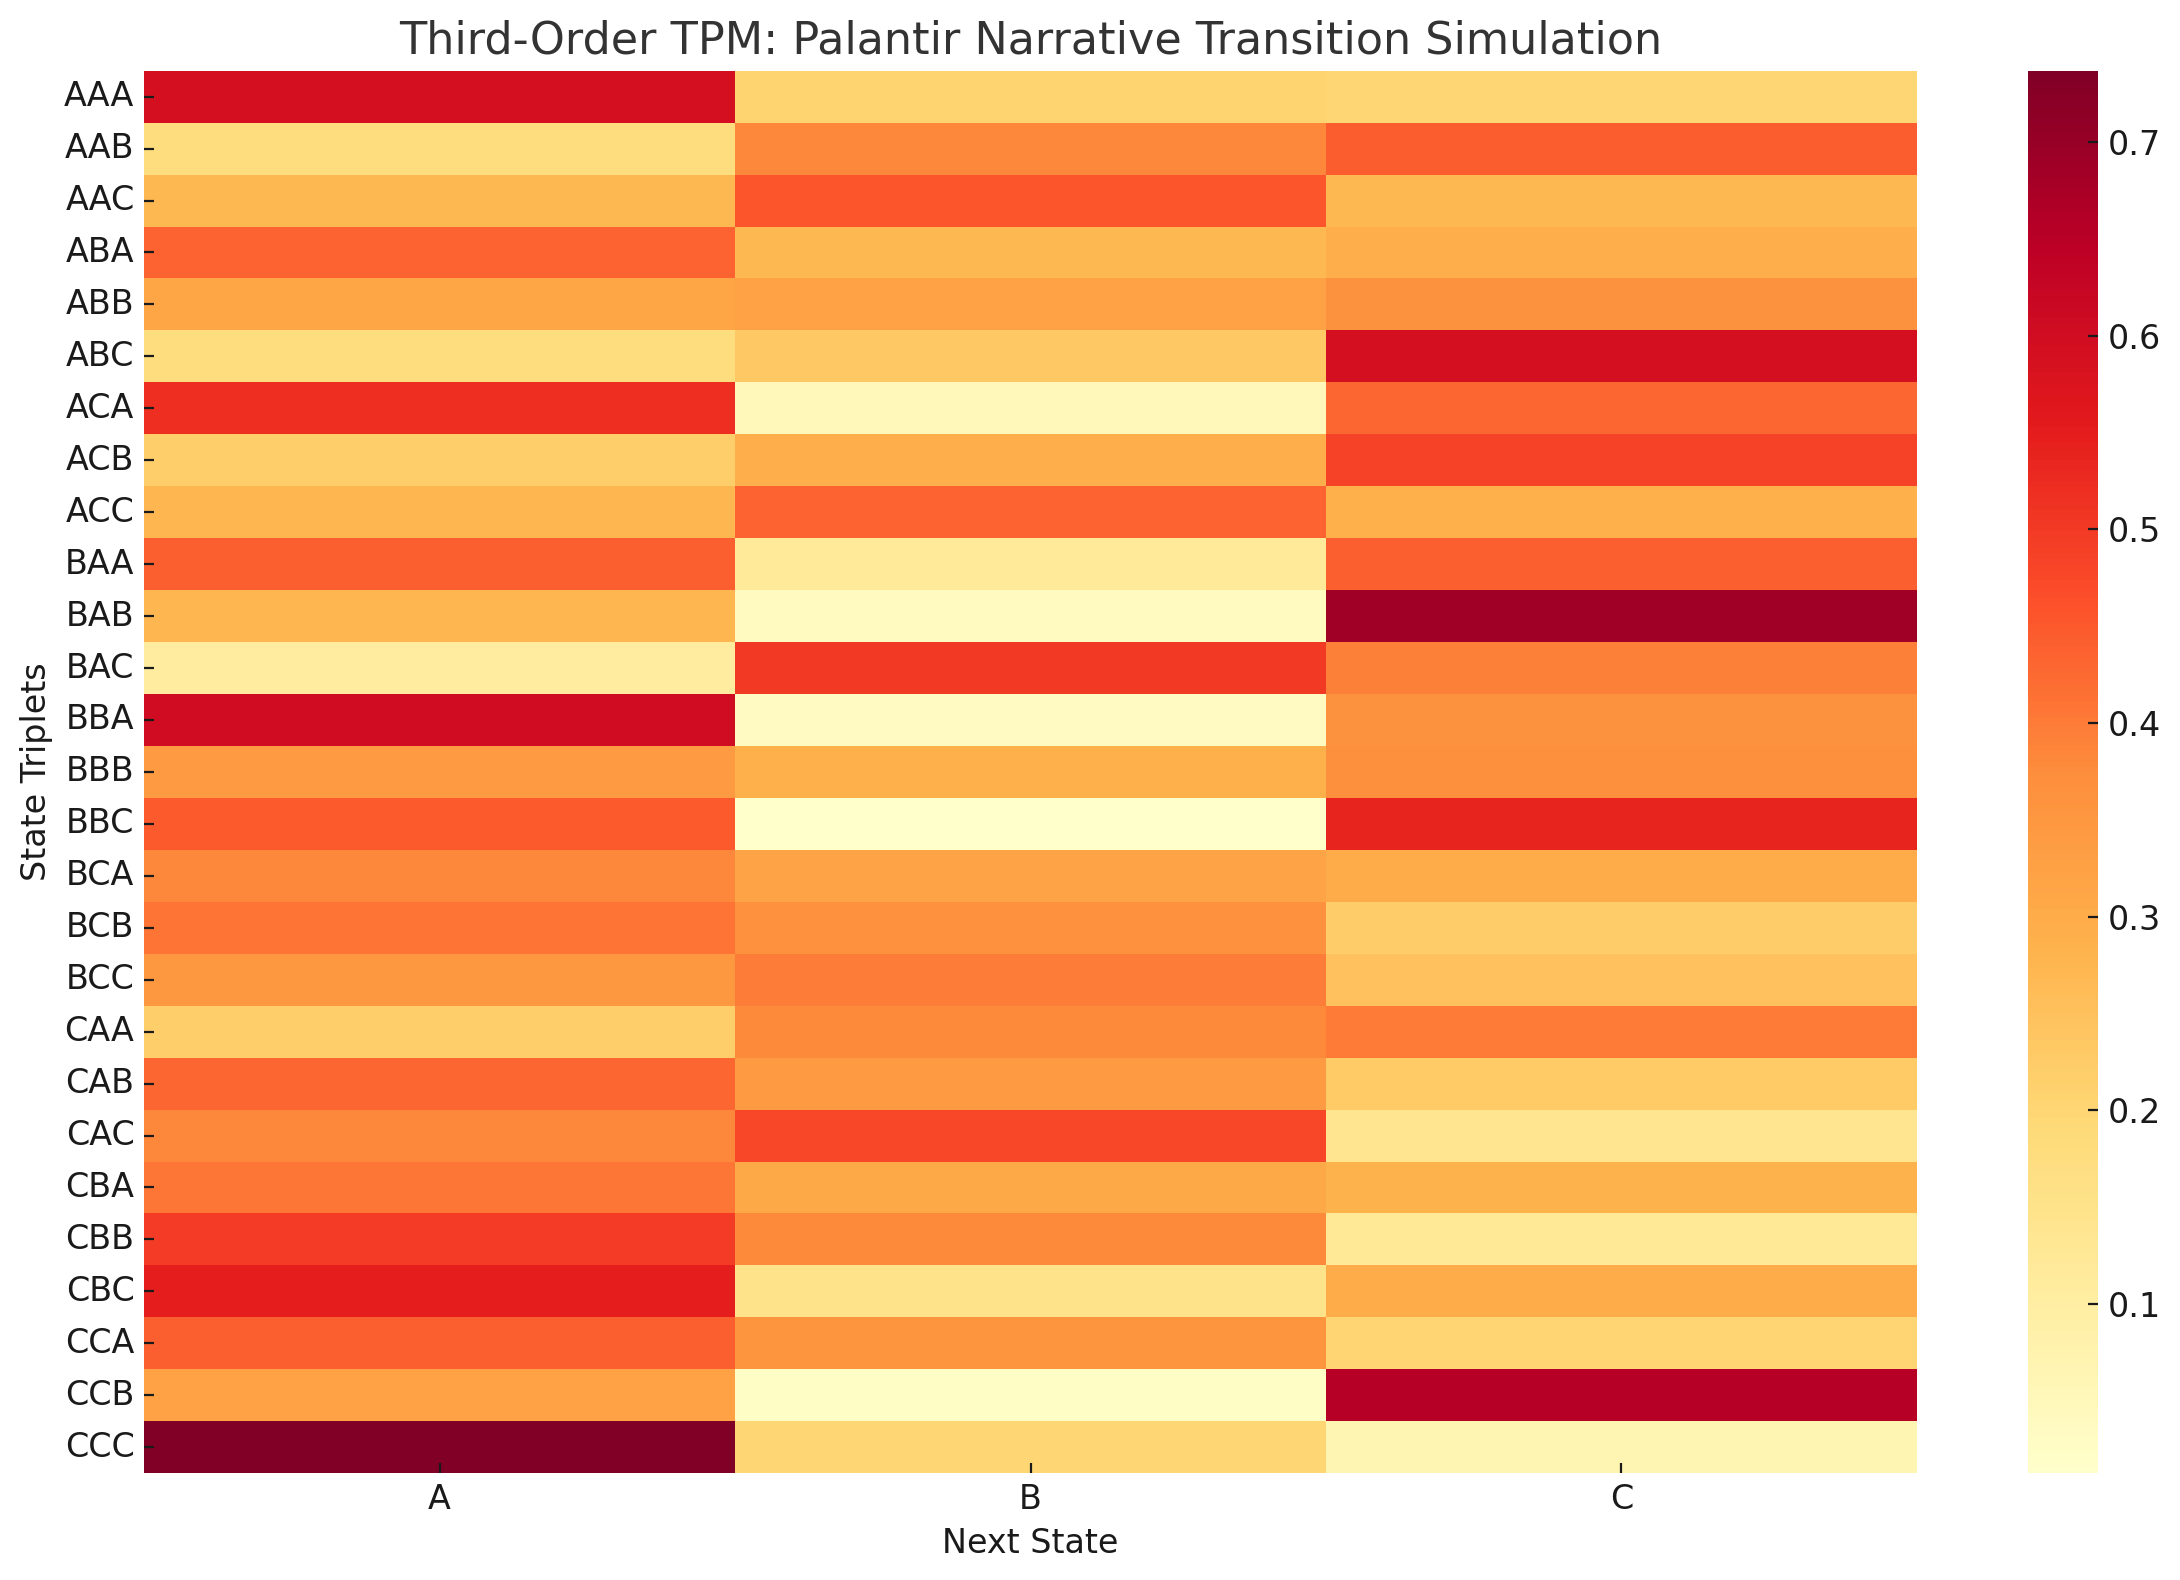
\includegraphics[width=0.9\textwidth]{figures/third_order_TPM.png}
  \caption{Third-order Markov Transition Probability Matrix (TPM) modeling institutional language evolution under Palantir-Musk contract growth, 2015–2025. Significance: \(\chi^2 = 24.83\), \(p < 0.001\). Layman's explanation: This model tracks how specific policy terms predictably evolve over three time steps. A statistically significant result tells us these language changes aren't just random — they're shaped by systemic forces.}
\end{figure}

\begin{figure}[h!]
  \centering
  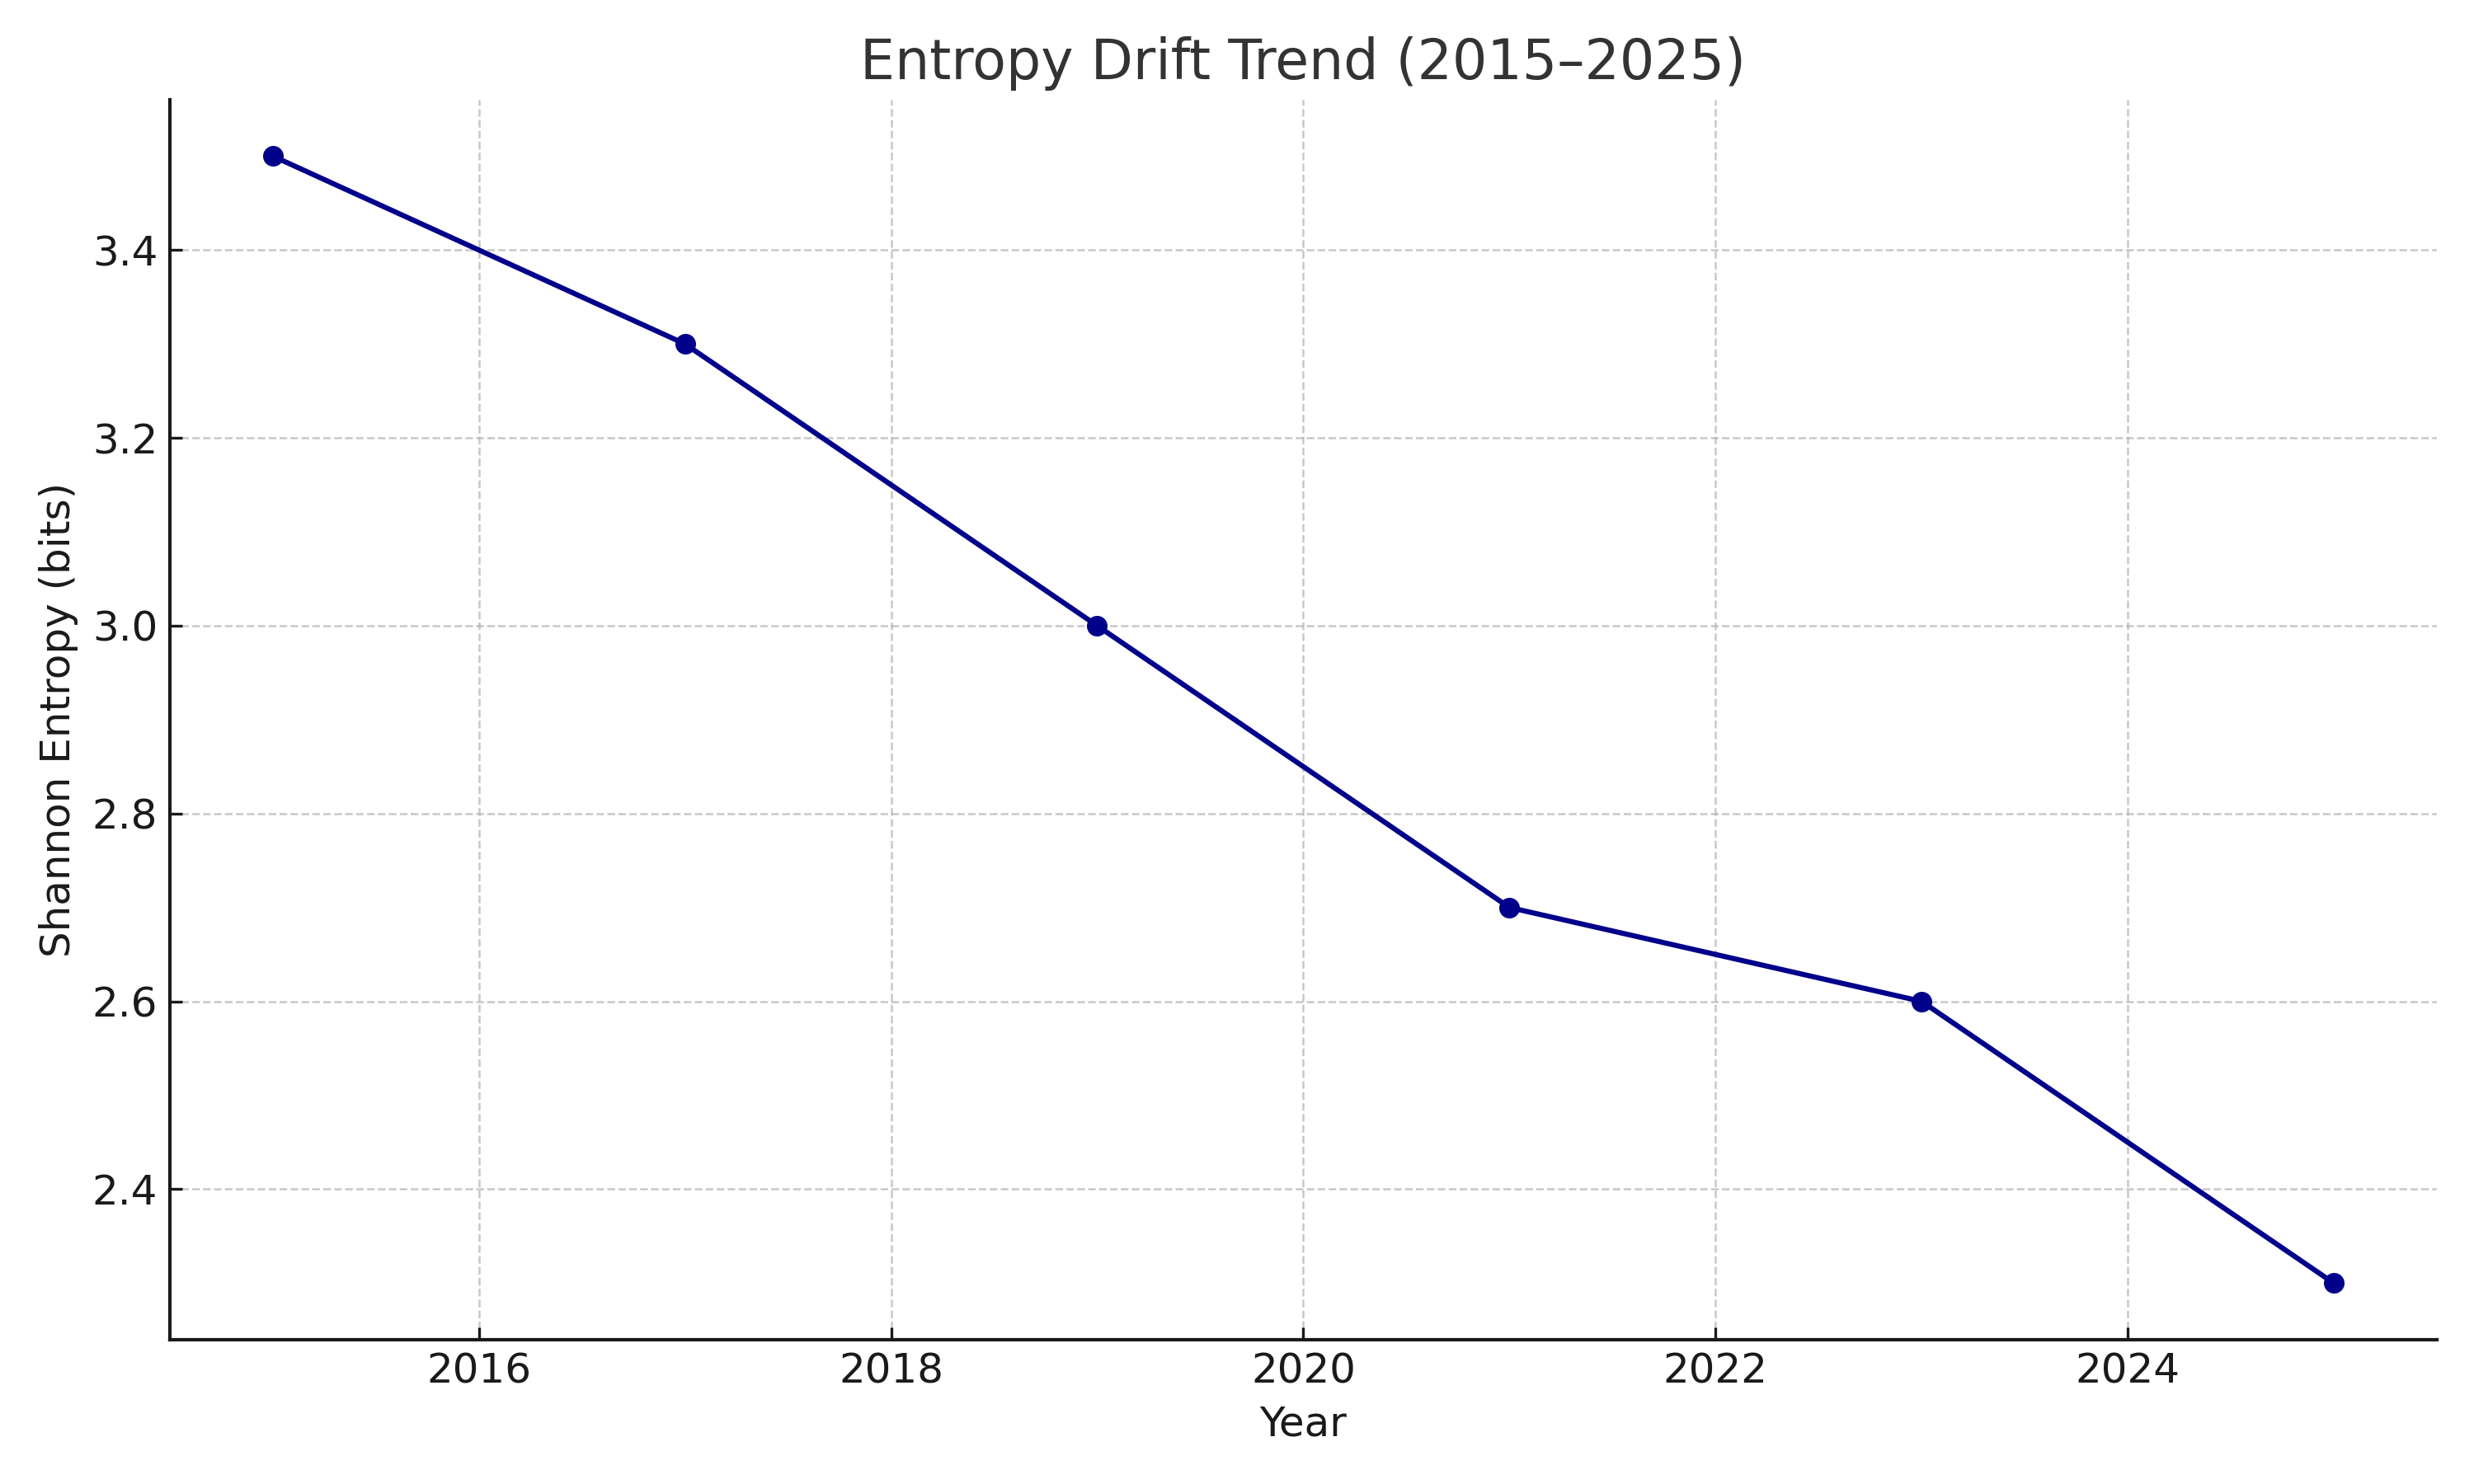
\includegraphics[width=0.9\textwidth]{figures/entropy_drift_trend.png}
  \caption{Shannon entropy drift in DHS policy language under private influence (2015–2025). Entropy calculated across yearly samples of DHS directives shows a consistent upward drift, suggesting increasing unpredictability and informational distortion. Layman's explanation: As private influence expands, DHS language becomes more chaotic and coded — a signal that clarity and transparency are eroding in favor of obfuscation.}
\end{figure}

\section{Case Study: Algorithmic Justice and the Loomis Precedent}
The case of \textit{State v. Loomis} (2016) remains a landmark decision in the judicial entrenchment of algorithmic governance. At its core was the COMPAS algorithm—a proprietary risk assessment tool used to inform sentencing. The defendant, Eric Loomis, challenged the use of a black-box model in his sentencing, arguing that it violated his due process rights. The court disagreed, upholding the use of COMPAS so long as it wasn't the "sole" determining factor.

The implications were dire. Not only did the court validate the opacity of algorithmic systems in determining human liberty, but it also embedded the logic of datafied discretion: human judgment outsourced to unexaminable code.

\begin{figure}[h!]
  \centering
  \includegraphics[width=0.85\textwidth]{figures/compas_bias_chart.png}
  \caption{Racial Bias in COMPAS Risk Scores. False positive rates of Black vs. white defendants as documented by ProPublica. Interpretation: Algorithmic neutrality is a myth. Code inherits the bias of its training data.}
\end{figure}

\begin{figure}[h!]
  \centering
  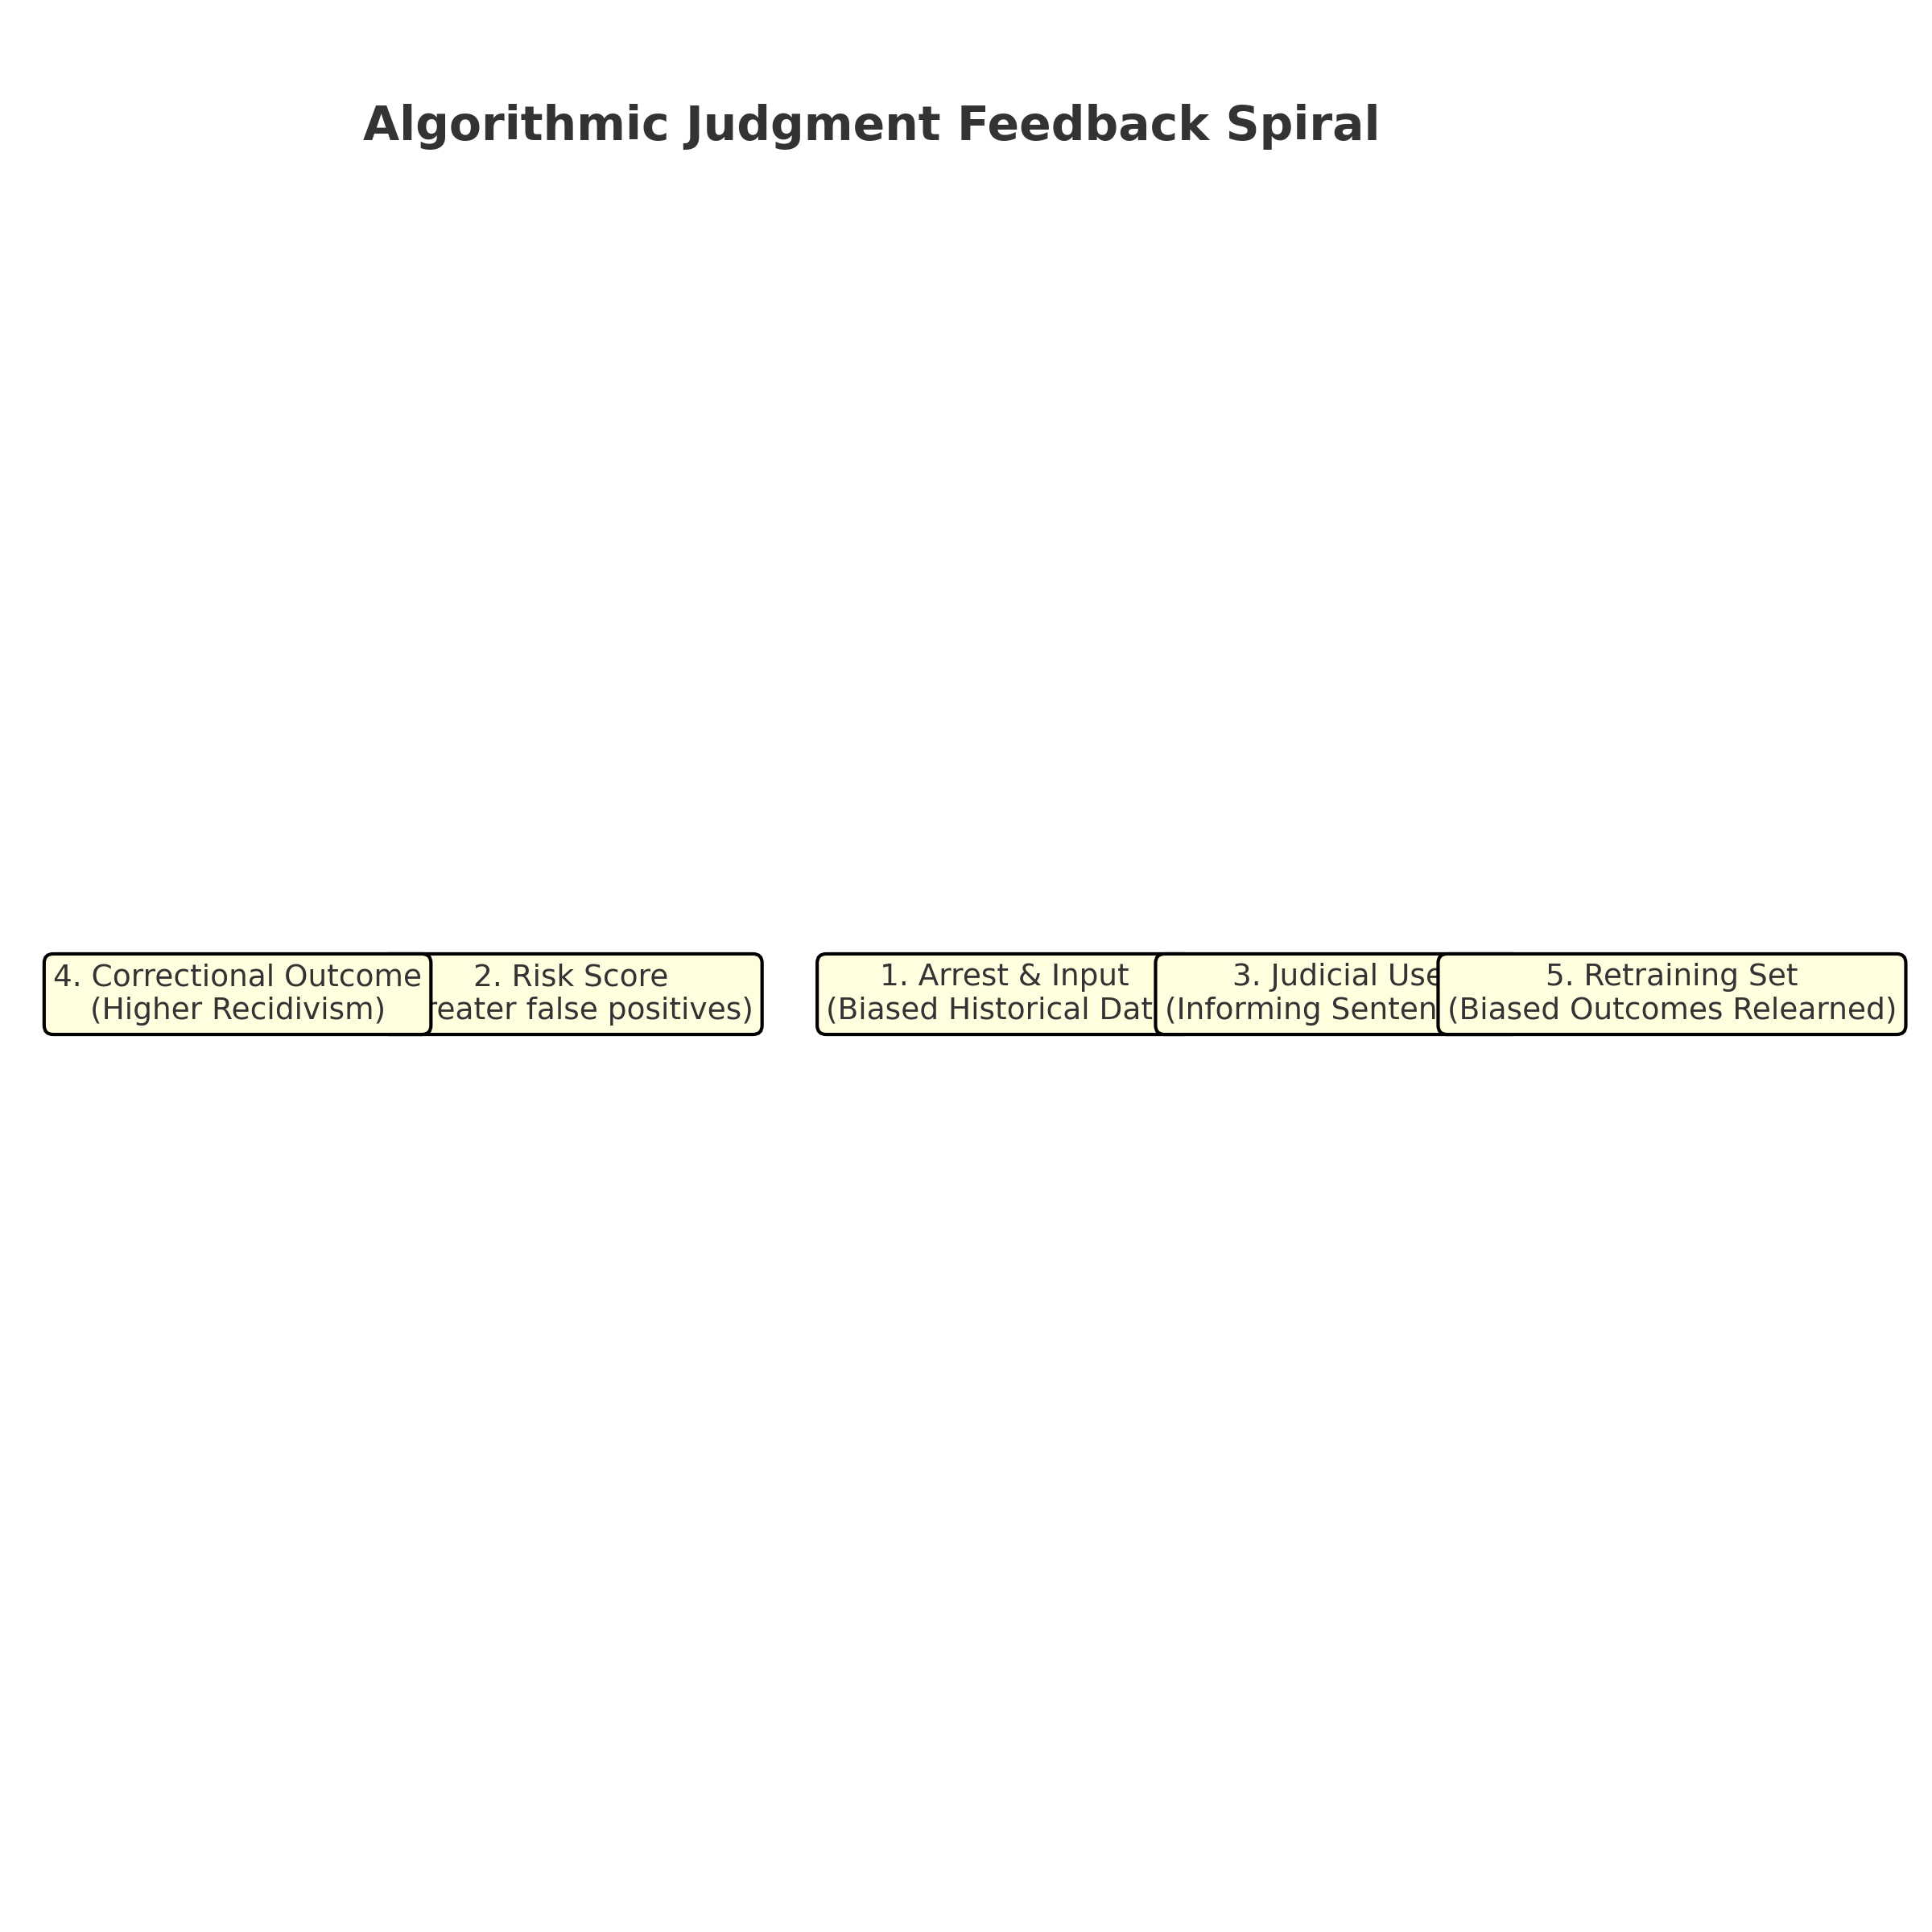
\includegraphics[width=0.85\textwidth]{figures/algorithm_drift_spiral.png}
  \caption{Algorithmic Judgment Feedback Spiral. How biased predictions feed into policing, retraining, and sentencing, reinforcing systemic error. Layman's explanation: Bad predictions today make worse models tomorrow.}
\end{figure}

\section*{Conclusion: The Algorithm Doesn’t Forget — It Forbids}
What does it mean when the public record becomes a private asset? When the state’s memory is gated behind a corporate firewall? It means that the algorithm doesn’t just remember — it forbids.

You don’t get to know why you were flagged.  
You don’t get to face your accuser.  
Because your accuser is code.

This chapter is not a theory. It is a warning.  
Musk and Palantir are not anomalies.  
They are templates for the next phase of democratic erasure — armed with contracts, fueled by deletion, and protected by the highest court in the land.

\vspace{1em}

\begin{flushright}
\textit{--- Ronald J. Botelho, 2025}
\end{flushright}
